\section{Conclusion}
\subsection{Summary}


\begin{frame}[t]{Motivation}
  Recent advances in Underwater Vehicle (UV) systems have enabled
  scientists and engineers to consider complex, multifaceted UV
  missions previously thought impractical or infeasible.

\alert{Thesis Goal}: Develop improved
  {\bf state estimation}, {\bf parameter identification}, and
  {\bf control} algorithms.
%    
    \begin{columns}
      \column{.45\textwidth}
\begin{center}
      \begin{figure}[htbp]
        \begin{center}
          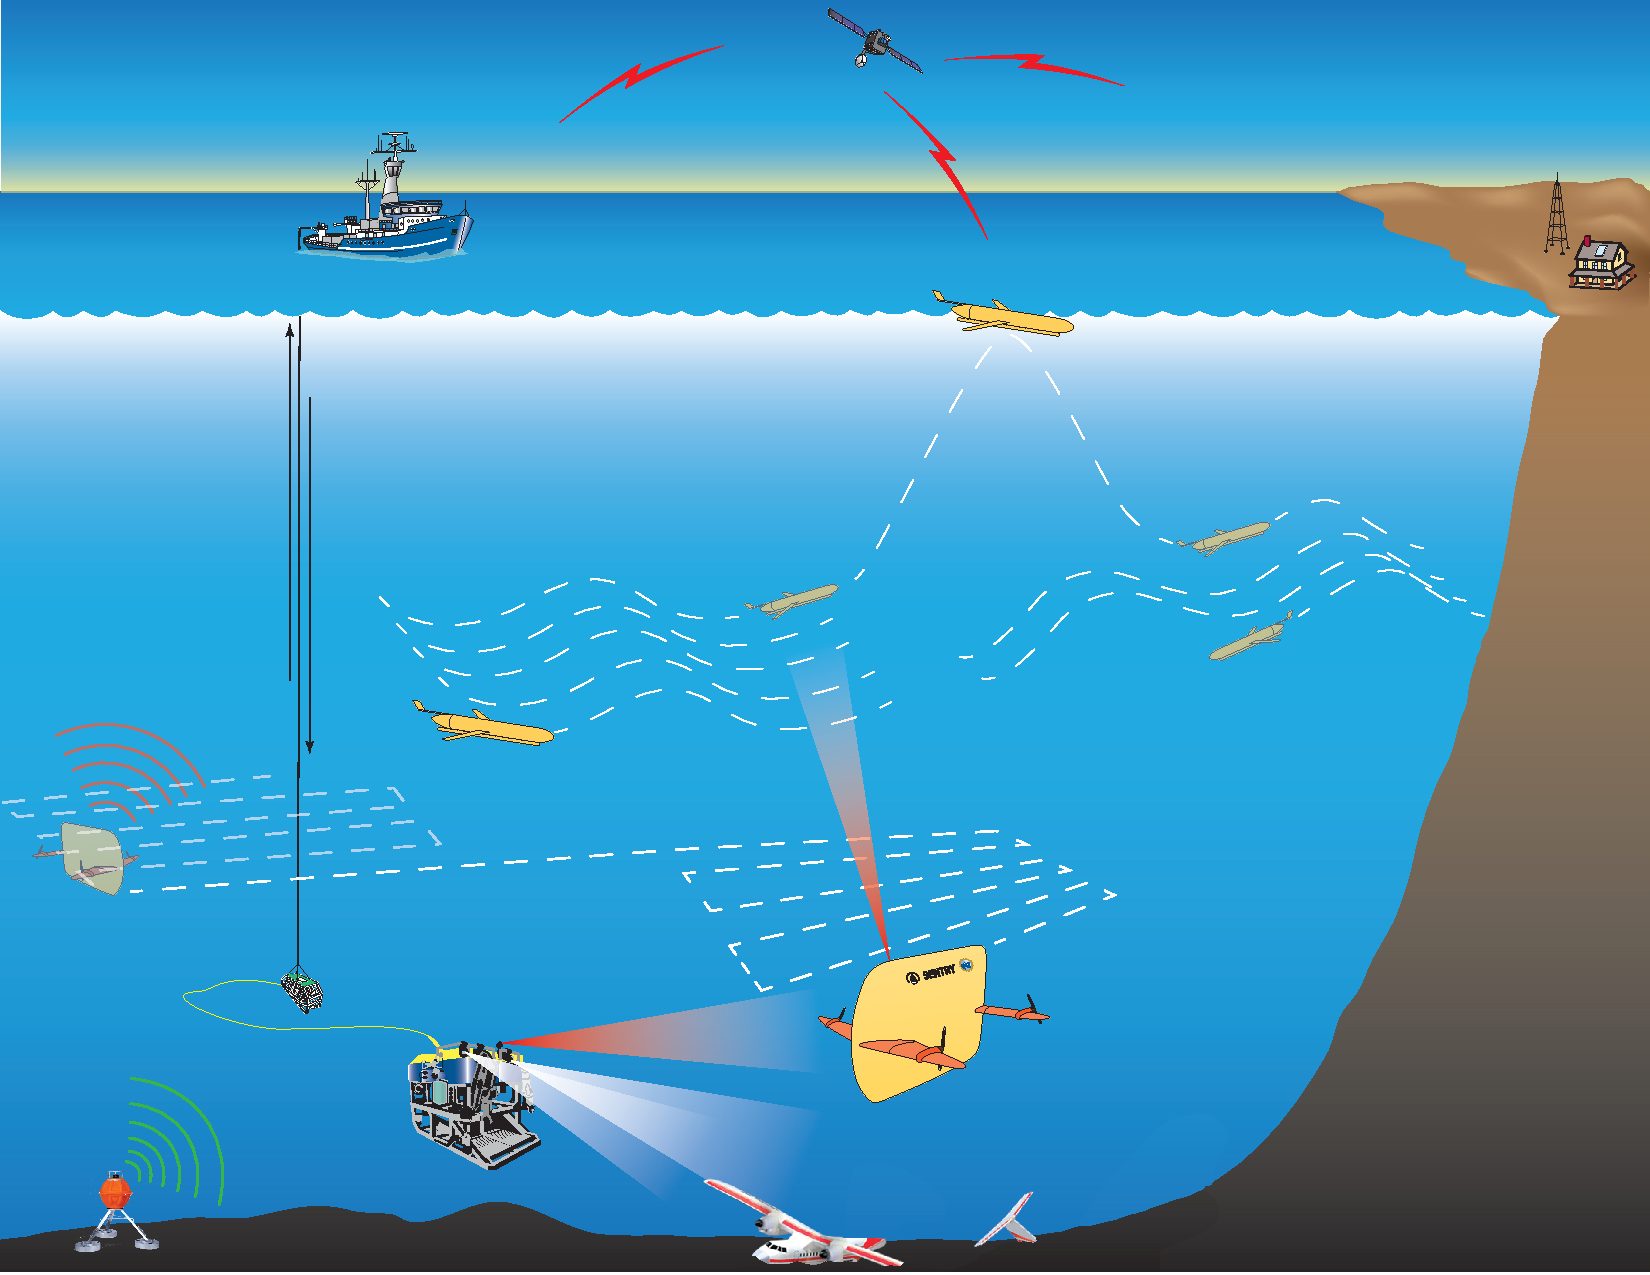
\includegraphics[width=1.1\textwidth]{./pres/images/Adaptive4}
%\caption{ Image credit: Paul Oberlander, WHOI. }
        \end{center}
      \end{figure}
    \end{center}
{\small Image credit: Paul Oberlander, WHOI.}

  \column{.55\textwidth}

  \begin{itemize}
  \item {\bf Improved State Estimation} algorithms can
    increase navigation accuracy while lowering UV cost.
  \item {\bf Improved Parameter Identification} algorithms enable
    remote operators to use forward simulation for mission planning
    and diagnose UV failure.
  \item {\bf Improved Control} algorithms enable increased precision
    of delicate or dynamic 6-degree-of-freedom
    (DOF) operation.
  \end{itemize}


 \end{columns}

\end{frame}


% \begin{frame}{Summary}
% %  Recent advances in Underwater Vehicle (UV) systems have enabled
% %  scientists and engineers to consider complex, multifacited UV
% %  missions previously thought impractical or impossible.

%   \alert{Thesis Goal}: Develop improved {\bf state estimation}, {\bf parameter
%     identification}, and {\bf control algorithms}.

% \vskip9pt    
% \vskip9pt    
% \vskip9pt    
%     \begin{columns}
%       \column{.5\textwidth}
% \alt<1>{}{    \begin{center}
%       \begin{figure}[htbp]
%         \begin{center}
%           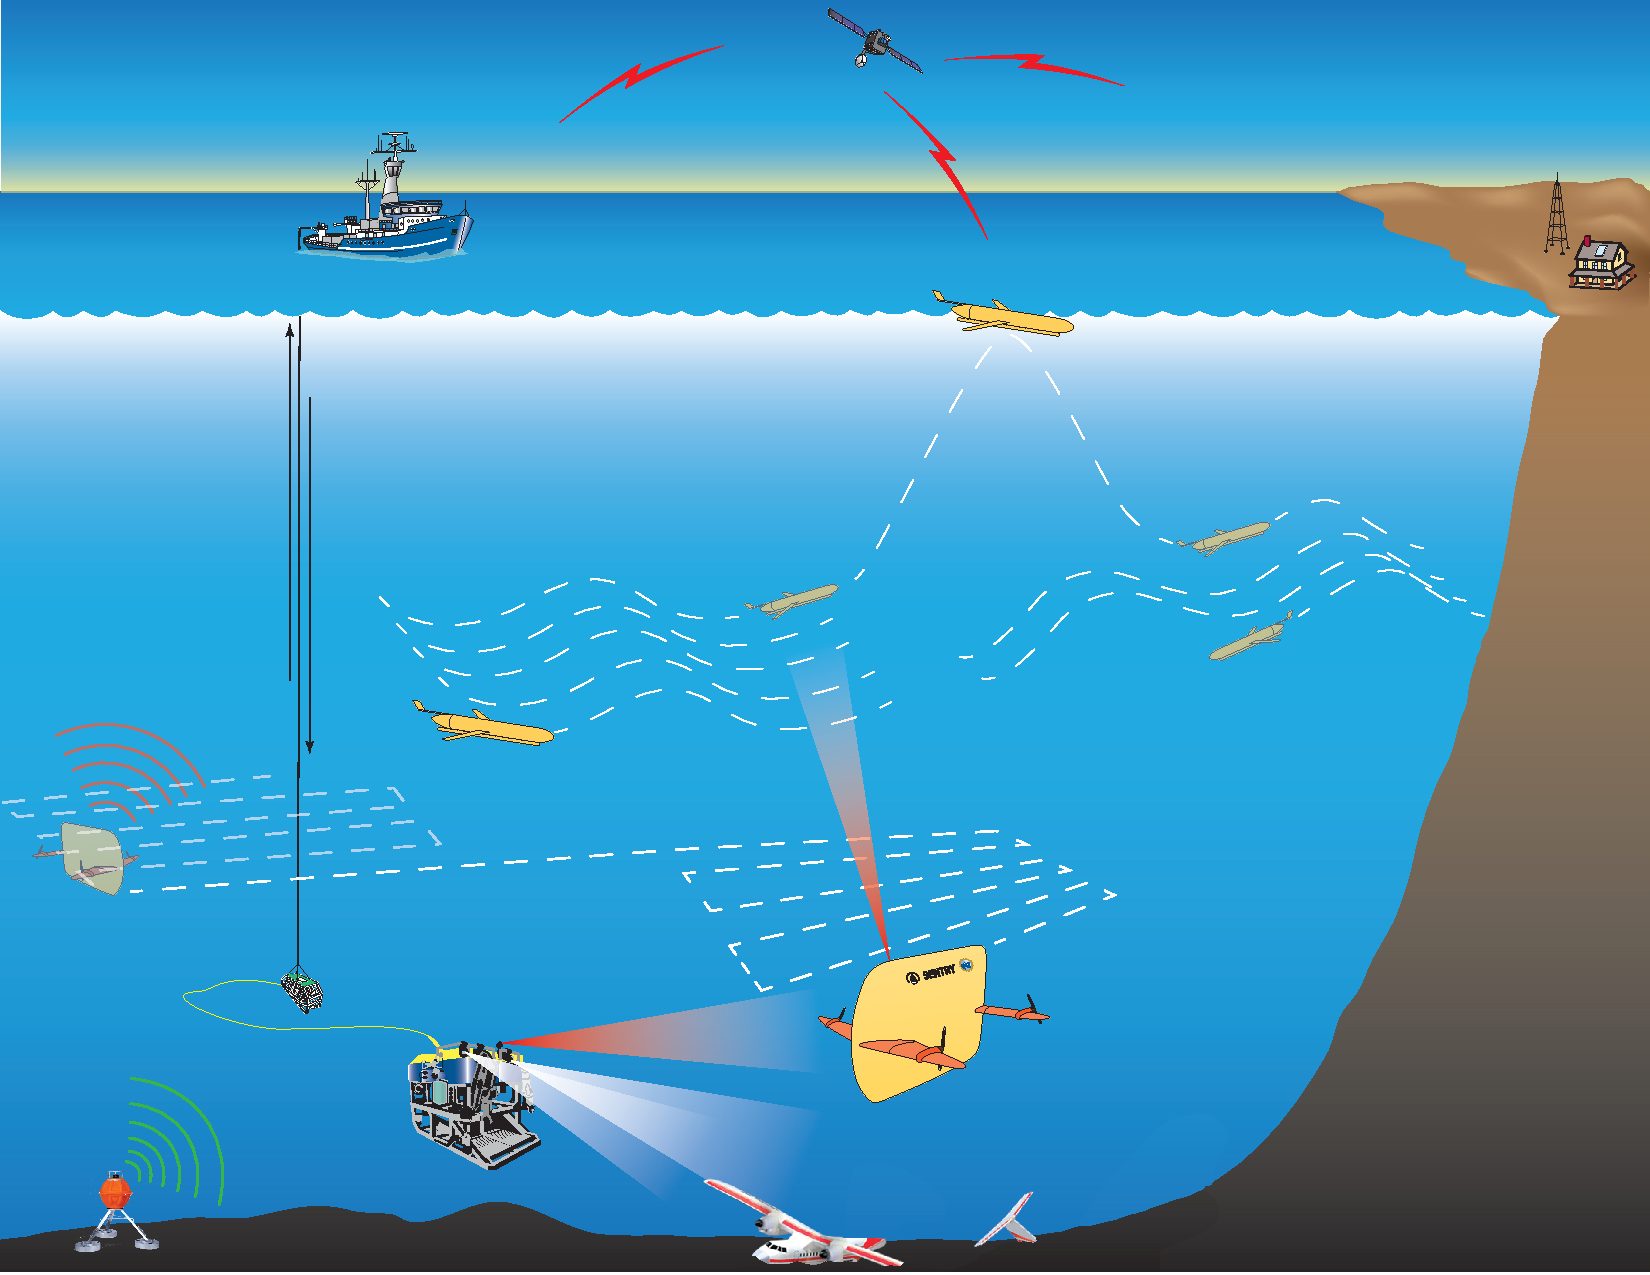
\includegraphics[width=\textwidth]{./pres/images/Adaptive4}
% %\caption{ Image credit: Paul Oberlander, WHOI. }
%         \end{center}
%       \end{figure}
%     \end{center}
% {\small Image credit: Paul Oberlander, WHOI.}}

%   \column{.5\textwidth}
% \vskip9pt
%   \uncover<2->{ The state estimation, adaptive identification, and
%     adaptive model-based control algorithms reported preform as well
%     as or better than current solutions.  
% \vskip9pt
% %They do so with while
% %    considering complicating features %such as underactuated vehicles or unmodeled thruster dynamics, which must
% %    which must be addressed before fielding such algorithms in the open ocean.
% \vskip9pt
% \vskip9pt
% \vskip9pt
% \vskip9pt}
%  \end{columns}

% \end{frame}


\subsection{Questions?}
\begin{frame}[t]{Questions?}
\begin{columns}
\column{.5\textwidth}
  \tableofcontents
\column{.5\textwidth}
  \begin{center}
\begin{figure}[htbp]  
  \begin{center}
    \includegraphics[width=40mm]{./pres/images/tophNereus}
  \end{center}
  \caption{McFarland and Nereus (WHOI) during field deployment in 2011.}
\end{figure}
\end{center}
\end{columns}

\end{frame}
